\documentclass[A1,landscape]{poster}
\newcommand{\onebf}{\ensuremath{\mathbf{1}}}
\newcommand{\Ibf}{\ensuremath{\mathbf{I}}}
\newcommand{\vbf}{\mathbf{v}}
\newcommand{\wbf}{\mathbf{w}}
\newcommand{\xbf}{\ensuremath{\mathbf{x}}}
\newcommand{\zerobf}{\ensuremath{{\mathbf 0}}}

\newcommand{\Dcal}{\ensuremath{\mathcal{D}}}
\newcommand{\Hcal}{\ensuremath{\mathcal{H}}}
\newcommand{\Lcal}{\ensuremath{\mathcal{L}}}
\newcommand{\Mcal}{\ensuremath{\mathcal{M}}}
\newcommand{\Ncal}{\ensuremath{\mathcal{N}}}
\newcommand{\Rcal}{\ensuremath{\mathcal{R}}}
\newcommand{\Scal}{\ensuremath{\mathcal{S}}}
\newcommand{\Tcal}{\ensuremath{\mathcal{T}}}
\newcommand{\Vcal}{\ensuremath{\mathcal{V}}}
\newcommand{\Xcal}{\ensuremath{\mathcal{X}}}
\newcommand{\Ycal}{\ensuremath{\mathcal{Y}}}

\newcommand{\Ebb}{\ensuremath{\mathbb{E}}}
\newcommand{\Nbb}{\ensuremath{\mathbb{N}}}
\newcommand{\Pbb}{\ensuremath{\mathbb{P}}}
\newcommand{\Rbb}{\ensuremath{\mathbb{R}}}

\newcommand{\N}{\Nbb}
\newcommand{\R}{\Rbb}
\newcommand{\Rpe}{\R_{+}^{*}}

\newcommand{\LB}{\left[}
\newcommand{\RB}{\right]}
\newcommand{\LC}{\left\{}
\newcommand{\RC}{\right\}}
\renewcommand{\RN}{\right\vert}
\newcommand{\LN}{\left\vert}
\newcommand{\LP}{\left(}
\newcommand{\RP}{\right)}

\newcommand{\ie}{{\it i.e.}\xspace}
\newcommand{\eg}{{\it e.g.}\xspace}
\newcommand{\resp}{{\it resp.}\xspace}
\newcommand{\wrt}{{\it w.r.t.}\xspace}
\newcommand{\iid}{{\it i.i.d.}\xspace}

\newcommand{\defeq}{\triangleq}

\newcommand{\indic}{\operatorname{I}}
\DeclareMathOperator*{\EE}{\Ebb}
\DeclareMathOperator*{\PP}{\Pbb}
\DeclareMathOperator*{\esssup}{\text{\rm esssup}}

\newcommand{\KL}{\operatorname{KL}}
\newcommand{\kl}{\operatorname{kl}}
\newcommand{\klmax}{\overline{\kl}}

\newcommand{\loss}{\ell}
\newcommand{\Risk}{\text{R}}
\newcommand{\RiskLoss}{\Risk^{\loss}}
\newcommand{\RiskLossp}{\Risk^{\loss'}}

\renewcommand{\P}{\pi}
\newcommand{\Q}{\rho}
\newcommand{\AQ}{\Q_{\Scal}}

\newcommand{\comp}{\operatorname{\mu}}
\newcommand{\uc}{{\tt u}}
\renewcommand{\aa}{{\tt a}}
\newcommand{\PhiUC}{\Phi_{\uc}}
\newcommand{\PhiA}{\Phi_{\aa}}
\newcommand{\PhiComp}{\Phi_{\comp}}

\newcommand{\vc}{{\tt vc}}
\newcommand{\rad}{{\tt rad}}

\newcommand{\distdistfro}{\distfro^{\boldsymbol{D}}}
\newcommand{\distdistltwo}{\distltwo^{\boldsymbol{D}}}
\newcommand{\distpathnorm}{\pathnorm^{\boldsymbol{D}}}
\newcommand{\distparamnorm}{\paramnorm^{\boldsymbol{D}}}
\newcommand{\distsumfro}{\sumfro^{\boldsymbol{D}}}
\newcommand{\distgap}{\gap^{\boldsymbol{D}}}
\newcommand{\distneural}{\neural^{\boldsymbol{D}}}

\newcommand{\riskdistfro}{\distfro^{\boldsymbol{R}}}
\newcommand{\riskdistltwo}{\distltwo^{\boldsymbol{R}}}
\newcommand{\riskpathnorm}{\pathnorm^{\boldsymbol{R}}}
\newcommand{\riskparamnorm}{\paramnorm^{\boldsymbol{R}}}
\newcommand{\risksumfro}{\sumfro^{\boldsymbol{R}}}
\newcommand{\riskgap}{\gap^{\boldsymbol{R}}}

\newcommand{\distfro}{\text{DistFro}}
\newcommand{\distltwo}{\text{DistL$_2$}}
\newcommand{\pathnorm}{\text{PathNorm}}
\newcommand{\paramnorm}{\text{ParNorm}}
\newcommand{\sumfro}{\text{SumFro}}
\newcommand{\gap}{\text{Gap}}
\newcommand{\neural}{\text{Neural}}


\usepackage{tikz}
\usepackage{color}
\usepackage{xcolor}
\usepackage{amssymb}
\usepackage{amsmath}
\usepackage{amsfonts}
\usepackage{mathtools}
\usepackage{xspace}
\usepackage[misc]{ifsym}
\usepackage{etoolbox}
\usepackage{subcaption}
\usepackage{caption}
\usepackage{graphicx}
\usepackage{enumitem}
\setlist[itemize,1]{labelsep=6.5mm}

\definetitlestyle{sampletitle}{width=\paperwidth}{
\node[] at (\titleposleft+6cm,\titleposbottom+3cm) {
\includegraphics[height=0.05\textheight]{figures/hcurien.png}};
\node[] at 
(\titleposleft+16cm,\titleposbottom+3.0cm) {
\includegraphics[height=0.04\textheight]{figures/irisa.png}};
\node[] at 
(\titleposleft+15cm,\titleposbottom+6.0cm) {
\includegraphics[height=0.04\textheight]{figures/inria.png}};
\node[] at (\titleposleft+6cm,\titleposbottom+6.0cm) {
\includegraphics[height=0.03\textheight]{figures/iuf.png}};
\node[] at (\titleposleft+8cm,\titleposbottom+9cm) {
\includegraphics[height=0.02\textheight]{figures/servicenow.pdf}};
\node[] at (\titleposleft+110cm,\titleposbottom+5cm) {\includestandalone[height=0.12\textheight]{figures/fig_poster_0}};
}
\usetitlestyle{sampletitle}

%%%%%%%%%%%%%%%%%%%%%%%%%%%%%%%%%%%%%%%%%%%%%%%%%%%%%%%%%%%%%%%%%%%%%%%%%%%%%%%

\settitle{%
    \vspace{-1.0cm} 
    \hspace{-28.9cm}\xscalebox{1.5}{
      \begin{center}
      {\Huge\color{blockblue}\bf\MakeUppercase{Leveraging PAC-Bayes Theory and Gibbs Distributions\\[0.2cm] for Generalization Bounds with Complexity Measures}}
      \end{center}
    }\\[1.2cm]
    
    \centering
    {\color{blockblue}\LARGE Paul Viallard\textnormal{\textsuperscript{1}, Rémi Emonet \textsuperscript{2,3,4}, Amaury Habrard\textsuperscript{2,3,4}, Emilie Morvant\textsuperscript{2}}, Valentina Zantedeschi\textsuperscript{5}}\\[0.4cm]
    \textsuperscript{1} Univ Rennes, Inria, CNRS IRISA - UMR 6074, F35000 Rennes, France \hspace{0cm} \textsuperscript{2} Université Jean Monnet Saint-Etienne, CNRS, Institut d Optique Graduate School,\\ Inria$^{3}$, Laboratoire Hubert Curien UMR 5516, F-42023, SAINT-ETIENNE, FRANCE  \textsuperscript{4} Institut Universitaire de France (IUF)\hspace{0cm} \\ \textsuperscript{5} ServiceNow Research
    \vspace{0.5cm}
}

%%%%%%%%%%%%%%%%%%%%%%%%%%%%%%%%%%%%%%%%%%%%%%%%%%%%%%%%%%%%%%%%%%%%%%%%%%%%%%%

\begin{document}

\maketitle

\begin{columns}
\column{0.4}
  \myblock[greyblock]{Notation {\normalsize (for classification and PAC-Bayesian bounds)}}{

\vspace{-1.4cm}
\begin{minipage}{.5\linewidth}
\begin{itemize}
    \item Input space $\Xcal$ and label space $\Ycal$
    \item Unknown distribution $\Dcal$ on $\Xcal\times\Ycal$
    \item Learning sample $\Scal{=}\{(x_i, y_i)\}_{i=1}^{m}{\sim}\Dcal^m$
    \item[] {\small ($\indic[a]\!=\!1$ if $a$ is true and $0$ otherwise)}
\end{itemize}
    \end{minipage} 
    \begin{minipage}{.55\linewidth}
    \begin{itemize}
        \item Hypothesis set $\Hcal$
        \item Distributions $\P$ and $\AQ$ on $\Hcal$
        \item True risk $\Risk_{\Dcal}(h)=\PP_{(x,y)\sim\Dcal}\LB h(x)\ne y\RB$
        \item Empirical risk $\Risk_{\Scal}(h){=}\frac{1}{m}\sum_{i=1}^{m}I\!\LB h(x_i){\ne} y_i\RB$
    \end{itemize}
  \end{minipage}

  \vspace{-0.0cm}
}

%%%%%%%%%%%%%%%%%%%%%%%%%%%%%%%%%%%%%%%%%%%%%%%%%%%%%%%%%%%%%%%%%%%%%%%%%%%%%%%

\myblock[greyblock]{1- Drawbacks of Typical Generalization Bounds}{

    \vspace{-1.5cm}

    {\bf Example:} Uniform convergence generalization bounds {\small (\eg, Rademacher bounds)}

    {\small For any $\Dcal$ on $\Xcal{\times}\Ycal$, for any set $\Hcal$, for any $\delta\in(0, 1]$, we have with probability at least $1-\delta$ over $\Scal\sim\Dcal^m$}
    \begin{align*}
      \forall h{\in}\Hcal,\ \ \Risk_{\Dcal}(h){-}\Risk_{\Scal}(h) \le \text{Rad}_{\Scal}(\Hcal){+}3\sqrt{\frac{\ln\frac{2}{\delta}}{2m}} \hspace{1.5cm}\text{{\small where $\displaystyle\text{Rad}_{\Scal}(\Hcal)=\EE_{\boldsymbol{\sigma}}\left[ \sup_{h\in\Hcal}\frac{1}{m}\sum_{i=1}^{m}\sigma_iI\!\LB h(x_i){\ne} y_i\RB \right]$}}
    \end{align*}
    

    \vspace{0.5cm}
    {\bf Worst-case bound}: constant w.r.t $h\in\Hcal$;\\
    complexity term determined by the theoretical framework considered\\
    {$\Rightarrow$} {\bf The upper bound is not representative of the gap} $\Risk_{\Dcal}(h) - \Risk_{\Scal}(h)$
}

%%%%%%%%%%%%%%%%%%%%%%%%%%%%%%%%%%%%%%%%%%%%%%%%%%%%%%%%%%%%%%%%%%%%%%%%%%%%%%%

\myblock[greyblock]{3- Comparison with the Literature}{

  \vspace{-2.2cm}

  \hspace{4.0cm}\xscalebox{1.0}{\begin{itemize}
    \item Comparison with two bounds adapted to our setting
    \begin{itemize}
    \item Using a prior $\alpha$-concentrated around the empirical risk, i.e., \\ $\mu: h, \Scal \mapsto \alpha\RiskLoss_{\Scal}(h)$ with $\RiskLoss_{\Scal}(h)=\frac{1}{m}\sum_{i=1}^{m}\loss(h, (\xbf, y))$
    \item Bounded cross-entropy $\loss(h, (\xbf,y)) {=} -\frac{1}{4}\ln(e^{-4}{+}(1{-}2e^{-4})h(\xbf)[y])$\\
    {\small where $h(\xbf)[y]$ is the probability assigned to the label $y$ by $h$}
    \end{itemize}

  \item {\bf Our bound is competitive for data-dependent priors}\\[-0.2cm]
  {\small (when $\omega$ depends on $\Scal' \sim \Dcal^{m'}$ with $m'=m$)}
  \end{itemize}}

  \vspace{-0.2cm}
  
  \begin{center}
  \includestandalone[width=0.83\linewidth]{figures/fig_poster_2}
  \end{center}

}

%%%%%%%%%%%%%%%%%%%%%%%%%%%%%%%%%%%%%%%%%%%%%%%%%%%%%%%%%%%%%%%%%%%%%%%%%%%%%%%

\column{0.6}
\myblock[greyblock]{2- Generalization Bounds with Arbitrary Complexity Measures}{

  \vspace{-2.0cm}
  
  {\bf Objective: Deriving generalization bounds with a complexity measure $\comp(h, \Scal)$ chosen by the user}

\begin{minipage}{.10\linewidth}
\end{minipage}
\hfill
\begin{minipage}{.34\linewidth}
  Let $\AQ$ and $\P$ be two Gibbs distributions\\[-0.5cm]
\begin{align*}
  \AQ(h) \propto \exp\LB-\comp(h, \Scal)\RB \quad\text{and}\quad \P(h) \propto \exp\LB-\omega(h)\RB
\end{align*}
\end{minipage}
\begin{minipage}{.46\linewidth}
\vspace{0cm}
\begin{center}
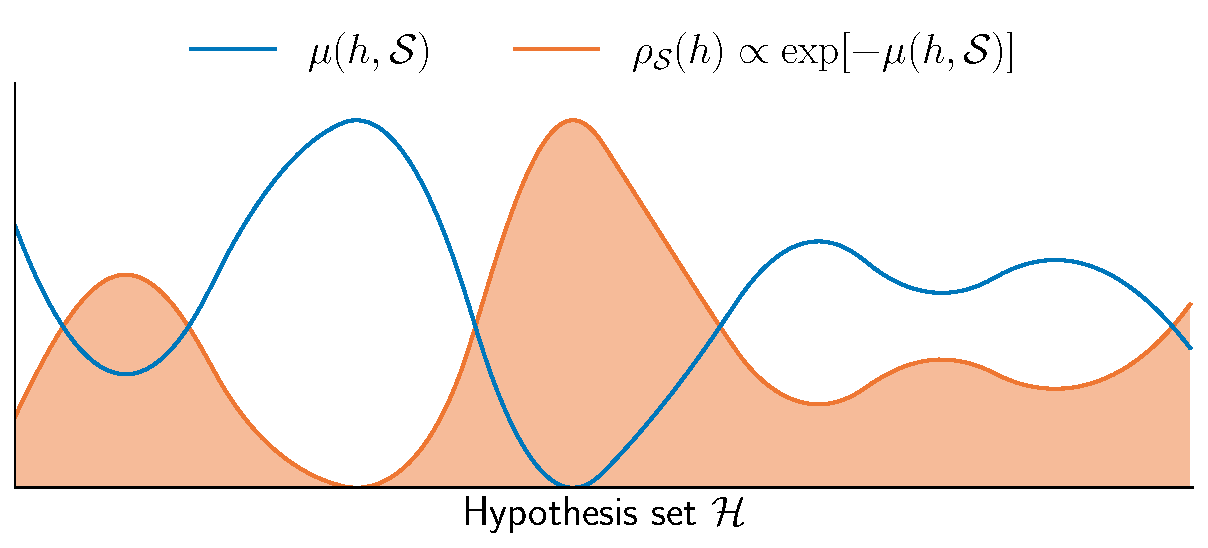
\includegraphics[scale=0.9]{figures/fig_poster_1.pdf}
\end{center}
\end{minipage}
\hfill
\begin{minipage}{.10\linewidth}
\end{minipage}

\vspace{0.5cm}

{\bf Our contribution:} {\normalsize For any $\Dcal$ on $\Xcal{\times}\Ycal$, for any set $\Hcal$, for any $\comp\!:\! \Hcal{\times}(\Xcal{\times}\Ycal)^m{\to}\R$, for any $\omega\!:\! \Hcal{\to}\R$, for any $\delta\!\in\!(0,1]$,}\\
\phantom{\bf Our contribution:} With probability at least $1{-}\delta$ over $\Scal{\sim}\Dcal^m$, $h'{\sim}\P$, $h{\sim}\AQ$ we have

\vspace{-0.5cm}
{\Large
\begin{align*}
  \vert\Risk_{\Dcal}(h){-}\Risk_{\Scal}(h)\vert \le \sqrt{\frac{1}{2m}\Big[[\comp(h'\!,\Scal){-}\omega(h')]-[\comp(h{,}\Scal){-}\omega(h)]+\ln\tfrac{8\sqrt{m}}{\delta^2} \Big]_{+}},\quad \text{{\normalsize where $[a]_+ = \max(0,a)$}}.
\end{align*}
}

\vspace{0.5cm}

{\bf Experiments with different complexity measures}, on MNIST {\small (+ FashionMNIST in the paper)}, \\ with All-Convolutional Network $h_{\wbf}$ (Springenberg et al., 2015) with weights $\wbf\!\in\!\R^d$ and $L$ layers
}

%%%%%%%%%%%%%%%%%%%%%%%%%%%%%%%%%%%%%%%%%%%%%%%%%%%%%%%%%%%%%%%%%%%%%%%%%%%%%%%

\begin{columns}

\column{0.4}

\column{0.3}
\myblock[greyblock]{4- Experiments on Regularized Risks}{
  \vspace{-1.5cm}

  \textbullet~Defining some ``norms'' $f(h,\Scal)$:\\[-0.2cm]

\begin{minipage}{.5\linewidth}
  \xscalebox{0.8}{  
    \textbullet~\mbox{$\distltwo(h, \Scal) = {\|\wbf{-}\vbf\|_{2}}$}\\[0.2cm]
    \textbullet~\mbox{$\distfro(h, \Scal) = \sum_{i=1}^{L} \|\wbf_{i}{-}\vbf_{i}\|_{2}$}\\[0.2cm]
    \textbullet~\mbox{$\paramnorm(h, \Scal) = {\sum_{i=1}^{L}\|\wbf_{i}\|_{2}^{2}}$}
  }
    \end{minipage} 
    \begin{minipage}{.5\linewidth}
  \xscalebox{0.8}{        
    \textbullet~\mbox{$\pathnorm(h, \Scal)= {\sum_{y\in\Ycal} h_{\wbf^2}(\onebf)[y]}$}\\[0.2cm]
    \textbullet~\mbox{$\sumfro(h, \Scal) = {L{[\prod_{i=1}^{L}\|\wbf_{i}\|_{2}^{2}]^{\frac1L}}}$}\\[0.2cm]
    \textbullet~\mbox{$\gap(h, \Scal) = {\vert\RiskLoss_{\Tcal}(h){-}\RiskLoss_{\Scal}(h)\vert}$}
      }
  \end{minipage}

  \vspace{0.5cm}
  {\small ($\vbf\in\R^d$ are random weights and $\Tcal$ is the test set)}
  

  \vspace{0.5cm}

  \textbullet~Experiments with $\beta$-regularized risks:\\[-0.0cm]
  \xscalebox{0.9}{
  \begin{center}
    $\mu(h,\Scal){=}f_{\beta}^{\boldsymbol{R}}(h, \Scal){=}{m(\beta\RiskLoss_{\Scal}(h){+}(1{-}\beta)f(h, \Scal))}$
  \end{center}
  }

  \vspace{0.2cm}
  \textbullet~{\bf Norms are not good predictors of }$\vert\Risk_{\Dcal}(h){-}\Risk_{\Scal}(h)\vert$ 


\vspace{0.9cm}
\includestandalone[width=1.0\linewidth]{figures/fig_poster_3}
}

%%%%%%%%%%%%%%%%%%%%%%%%%%%%%%%%%%%%%%%%%%%%%%%%%%%%%%%%%%%%%%%%%%%%%%%%%%%%%%%

\column{0.3}

\myblock[greyblock]{\xscalebox{0.95}{\mbox{5- Experiments with Neural Complexities}}}{

\vspace{-2.0cm}

  \begin{itemize}
    \item Hypothesis $h_{SGD}$ learned with SGD
    \item Additional ``norm'' $\neural(h,\Scal)$\\ {\normalsize (Feed-forward neural network learned to predict $\vert\Risk_{\Dcal}(h){-}\Risk_{\Scal}(h)\vert$)}
    \item Experiments with  
  \begin{align*}
    \mu(h, \Scal) {=} f^{\boldsymbol{D}}(h,\Scal) {=} m\vert f(h,\Scal){-}f(h_{\text{SGD}},\Scal)\vert \text{ and } \omega(h){=}0
  \end{align*}
    \item {\bf Neural complexities help tightening the bounds}
  \end{itemize}

  \vspace{0.5cm}
  \includestandalone[width=1.0\linewidth]{figures/fig_poster_4}

  \vspace{-1.0cm}
}

\begin{columns}

%%%%%%%%%%%%%%%%%%%%%%%%%%%%%%%%%%%%%%%%%%%%%%%%%%%%%%%%%%%%%%%%%%%%%%%%%%%%%%%

\column{0.7}
\column{0.3}
\myblock[greyblock]{References}{

\vspace{-2.0cm}

  {\footnotesize Gintare Karolina Dziugaite and Daniel M. Roy. Data-dependent PAC-Bayes priors via differential}\\[-0.5cm]
  {\footnotesize privacy. NeurIPS, 2018}\\[-1.8cm]

  {\footnotesize Guy Lever, François Laviolette, and John Shawe-Taylor. Tighter PAC-Bayes bounds through}\\[-0.5cm]
  {\footnotesize distribution-dependent priors. Theoretical Computer Science, 2013}\\[-1.8cm]

  {\footnotesize Jost Tobias Springenberg, Alexey Dosovitskiy, Thomas Brox, and Martin Riedmiller. Striving for}\\[-0.5cm]
  {\footnotesize Simplicity: The All Convolutional Net. ICLR – Workshop Track, 2015.}

}

\end{columns}

\end{columns}

\end{columns}

\end{document}
